\label{sec:intro}


% \noindent {\bf LG}

As we try to duplicate the successes of current deep convolutional architectures in the 3D domain, we face a fundamental representational issue. Extant deep net architectures for both discriminative and generative learning in the signal domain are well suited to data that is regularly sampled, such as images, audio, or video. However, most common 3D geometry representations, such as 2D meshes or point clouds are not regular structures and do not easily fit into architectures that exploit such regularity for weight sharing, etc.  That is why the majority of extant works on using deep nets for 3D data resort to either volumetric grids or collections of images (2D views of the geometry). Such representations, however, lead to difficult trade offs between sampling resolution and net efficiency. Furthermore, they enshrine quantization artifacts that obscure natural invariances of the data under rigid motions, etc.
\begin{figure}[t!]
	\centering
	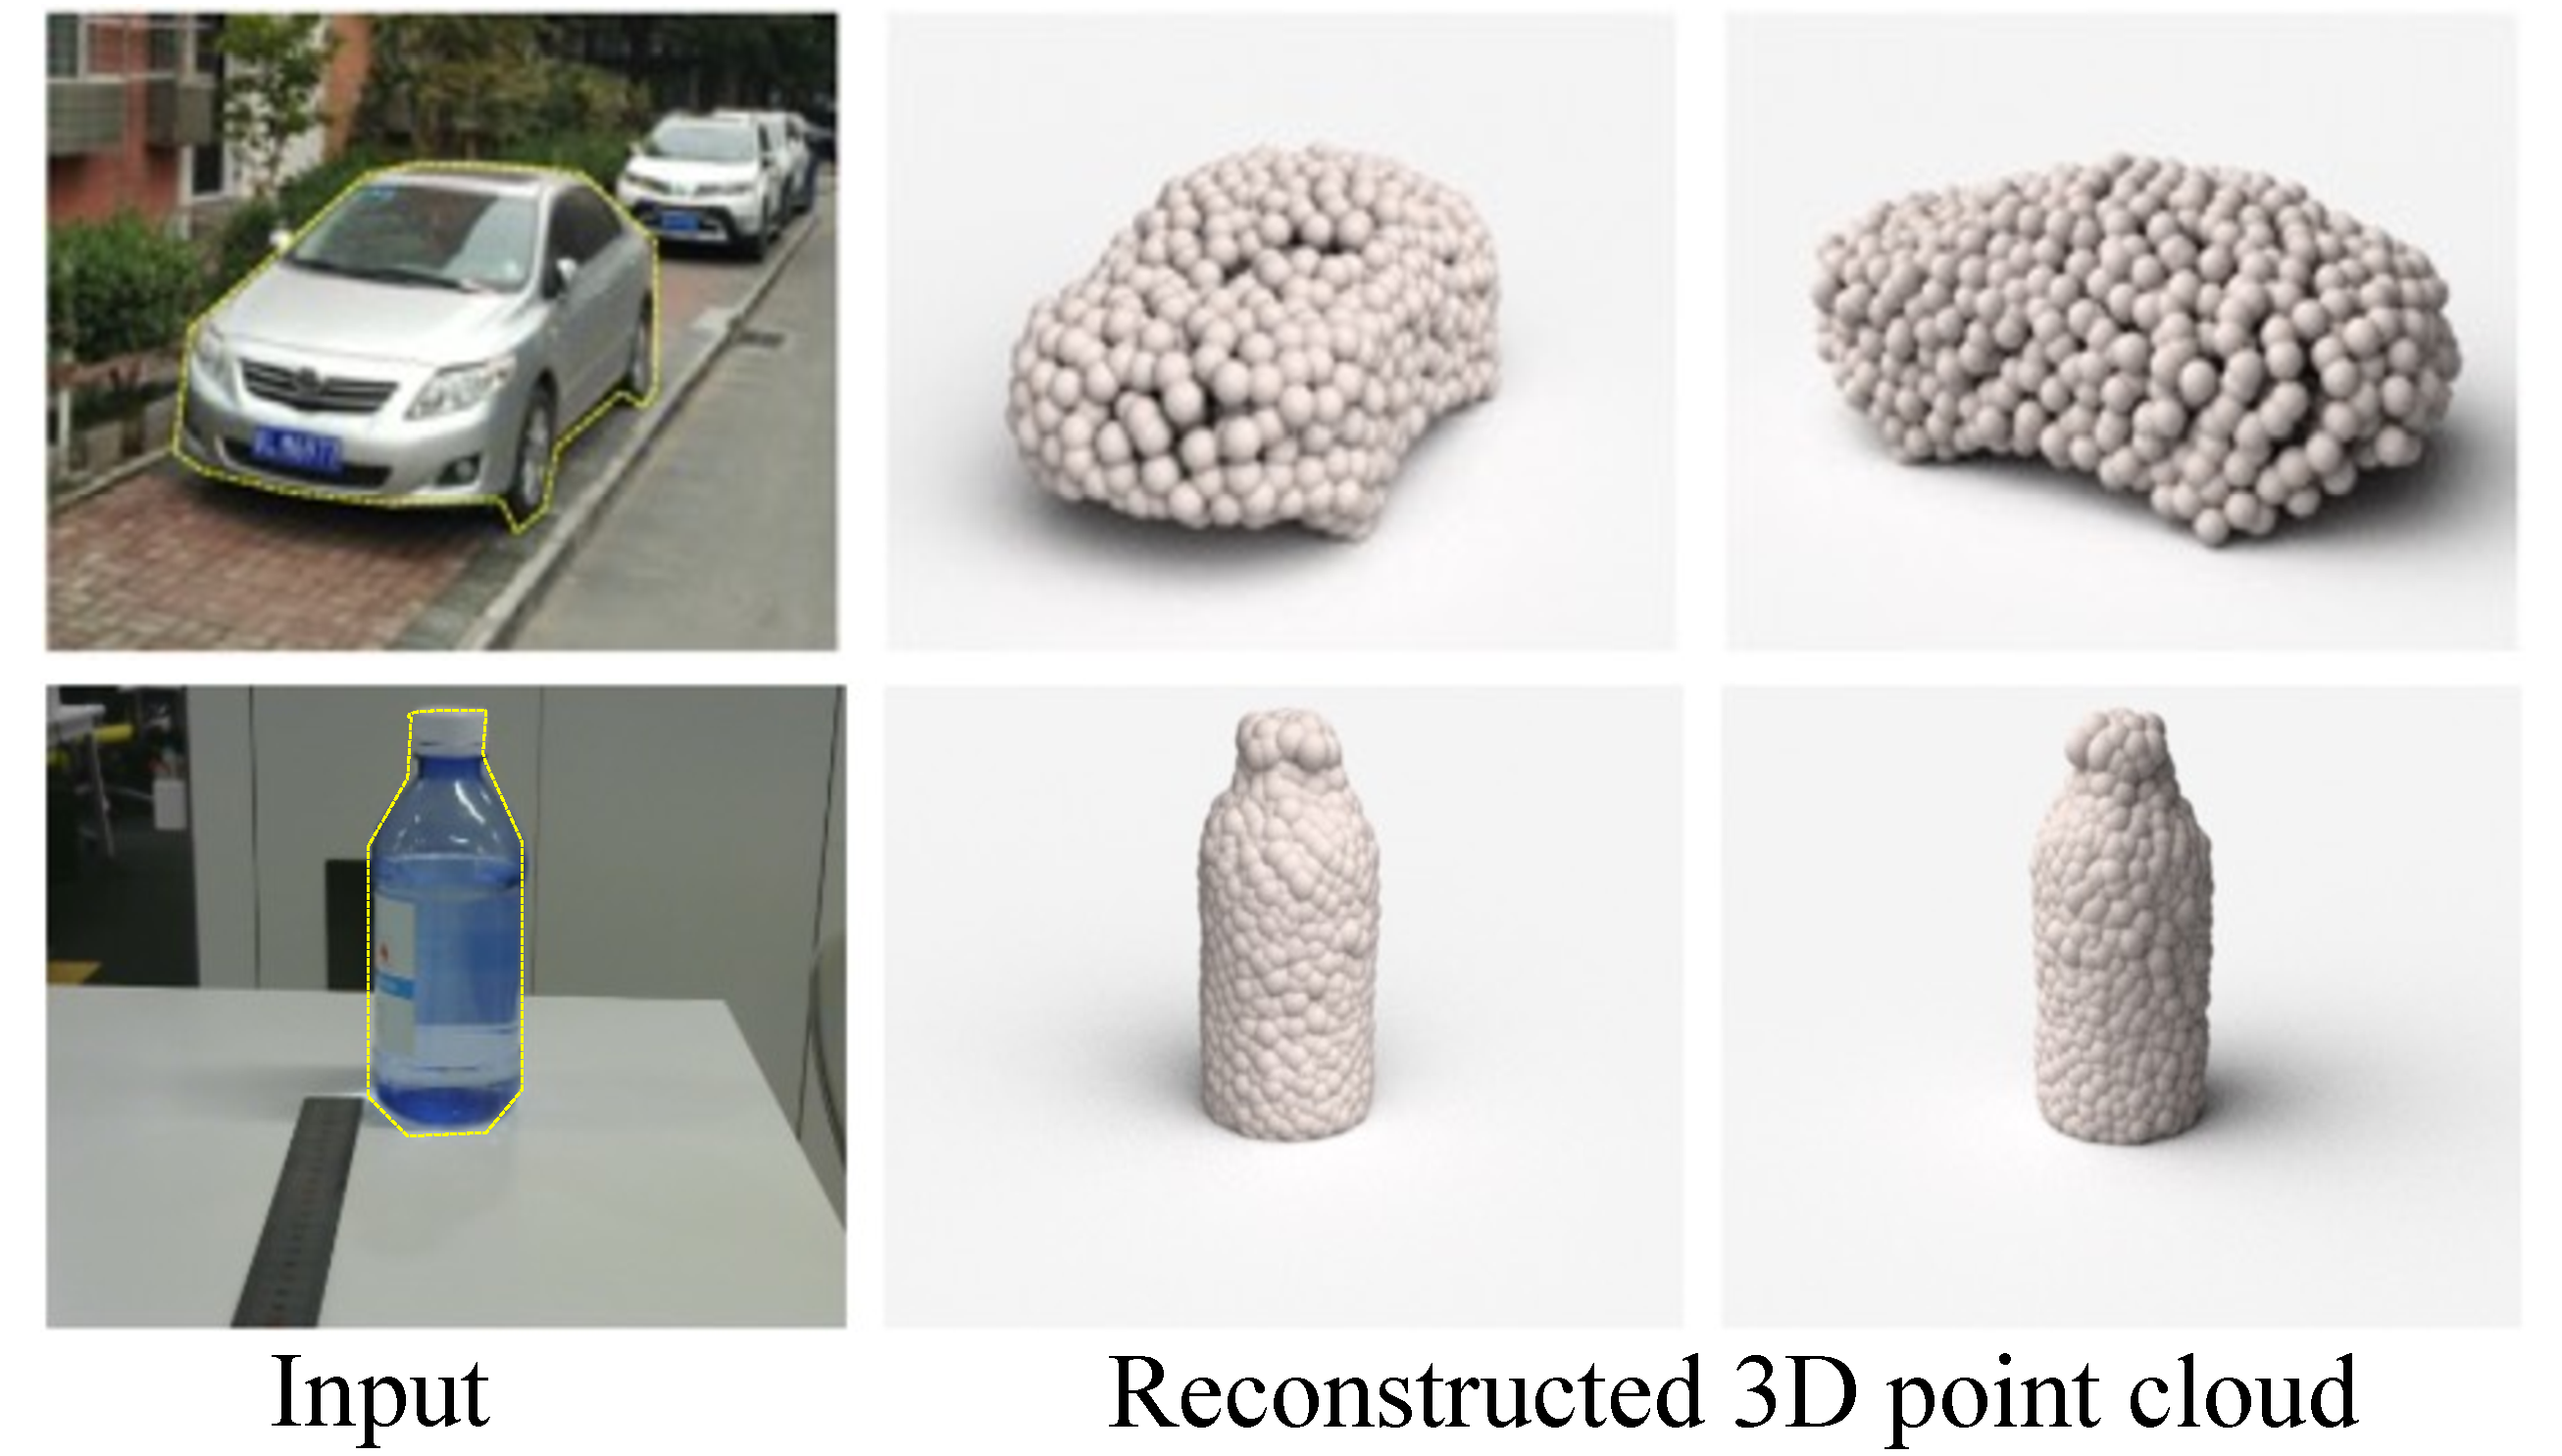
\includegraphics[width=\linewidth]{./fig/realworld2.pdf}
	\caption{A 3D point cloud of the {\bf complete} object can be reconstructed from a single image. Each point is visualized as a small sphere. The reconstruction is viewed at two viewpoints ($0^{\circ}$ and $90^{\circ}$ along azimuth). A segmentation mask is used to indicate the scope of the object in the image.}
	\label{fig:teaser}
	\vspace{-1em}
\end{figure}

In this paper we address the problem of generating the 3D geometry of an object based on a single image of that object. We explore generative networks for 3D geometry based on a point cloud representation. A point cloud representation may not be as efficient in representing the underlying continuous 3D geometry as compared to a CAD model using geometric primitives or even a simple mesh, but for our purposes it has many advantages, A point cloud is a simple, uniform structure that is easier to learn, as it does not have to encode multiple primitives or combinatorial connectivity patterns. In addition, a point cloud allows simple manipulation when it comes to geometric transformations and deformations, as connectivity does not have to be updated. Our pipeline infers the point positions in a 3D frame determined by the input image and the inferred viewpoint position.



Given this unorthodox network output, one of our challenges is how to measure loss during training, as the same geometry may admit different point cloud representations at the same degree of approximation. Unlike the usual $L_2$ type losses, we use the solution of a transportation problem based on the Earth Mover's distance (EMD), effectively solving an assignment problem. We exploit an approximation to the EMD to provide speed as well as ensure differentiability for end-to-end training.

Our approach effectively attempts to solve the ill-posed problem of 3D structure recovery from a single projection using certain learned priors. The network has to estimate depth for the visible parts of the image and hallucinate the rest of the object geometry, assessing the plausibility of several different completions. From a statistical perspective, it would be ideal if we can fully characterize the landscape of the ground truth space, or be able to sample plausible candidates accordingly. If we view this as a regression problem, then it has a rather unique and interesting feature arising from inherent object ambiguities in certain views. These are situations where there are multiple, equally good 3D reconstructions of a 2D image, making our problem very different from classical regression/classification settings, where each training sample has a unique ground truth annotation. In such settings the proper loss definition can be crucial in getting the most meaningful result.

Our final algorithm is a conditional sampler, which samples plausible 3D point clouds from the estimated ground truth space given an input image. Experiments on both synthetic and real world data verify the effectiveness of our method. % Since the label of our data is a point cloud, it is unclear how to conduct discriminative.
%We propose an extremely simple and parameter-free discriminative algorithm to train this sampler, by tactfully wrapping the EMD loss with a $\min$ function. This wrapped loss function (named MoN loss) can be trained almost as efficiently and easily as the vanilla loss. 
Our contributions can be summarized as follows:
\bitem
  \item We are the first to study the point set generation problem by deep learning; 
  \item On the task of 3D reconstruction from a single image, we apply our point set generation network and significantly outperform state of the art;
  \item We systematically explore issues in the architecture and loss function design for point generation network;
  \item We propose a principled formulation and solution to address the groundtruth ambiguity issue for the 3D reconstruction from single image task.
\eitem

% \quad
% 
% 
% \noindent {\bf HS}
% 
% Most previous generation models in deep learning output volumetric forms; however, we represent a 3D shape as a point cloud, i.e., a set of coordinates in $\R^3$. Compared with volumetric representations,
% %as previously used in~\cite{wu20153d,choy20163d,yumer2016learning}, 
% points are more friendly to geometric transformations and algebraic operations such as interpolation and extrapolation. Compared with primitive-based representations such as geons~\cite{biederman1987recognition} or polygonal meshes, point cloud is more flexible in approximating any shapes; in addition, it is in a more canonical form because no connectivity is involved\footnote{Different tessellations of points may generate almost identical shapes with very different connectivity.}, thus simpler to be learned. 
% % However, it is unclear how to conduct deep learning to generate a modestly sized point set.
% 
% We use a learning-based approach to regress the point clouds from a single image. However, as an exclusive property of this learning problem, the groundtruth shape of an input image is not unique --- the estimation of the depth for visible parts is underdetermined, and the completion of invisible parts is through hallucination. Certain priors must be added so that some solutions are more plausible than others. In a statistical perspective, it would be ideal if we can fully characterize the landscape of the groundtruth space, or be able to sample plausible candidates accordingly. This inherent property makes our problem very different from classical regression/classification settings, where each training sample has a unique groundtruth annotation. 
